\documentclass[14pt]{matmex-diploma-custom}

\usepackage{mathtools}
\usepackage{graphicx}
\usepackage{multicol}
\usepackage{multirow}
\usepackage{tabularx}
\usepackage{array}

\newcolumntype{M}[1]{>{\centering\arraybackslash}m{#1}}

\graphicspath{{pictures/}}
\DeclareGraphicsExtensions{.pdf,.png,.jpg}

\begin{document}

\filltitle{ru}{
    chair              = {Математическое обеспечение и администрирование \\ информационных систем \\ \vspace{5mm} Системное программирование},
    group              = {18Б.10-мм},
    title              = {Реализация операций линейной алгебры на графическом процессоре с использованием F\#},
    type               = {practice},
    author             = {Черников Артем Александрович},
    supervisorPosition = {к.ф.-м.н., доцент кафедры информатики СПбГУ},
    supervisor         = {Григорьев С. В.},
}
\maketitle
\tableofcontents

\section*{Введение}
\paragraph{} Граф --- одна из важнейших абстрактных структур данных в информатике. Алгоритмы, использующие графы, применяются в таких областях, как биоинформатика \cite{Georganas}, компьютерные сети и социальные сети \cite{Riedy}. Было показано, что из-за своей простоты и общности графы являются мощными инструментами для моделирования сложных задач \cite{Bergamini}. Поэтому алгоритмы на графах стали одними из фундаментальных единиц в теоретической информатике\footnote{Под термином "информатика" в данном случае подразумевается англоязычный термин "computer science"}, предоставив информационные ресурсы для исследований в различных областях, таких как, например, комбинаторная оптимизация, теория сложности и топология. Алгоритмы на графах были адаптированы и реализованы военными, коммерческими предприятиями и исследователями в академических кругах и стали незаменимыми для управления электросетью, телефонными системами и, конечно же, компьютерными сетями.

Параллельные алгоритмы на графах, как известно, сложно реализовать и оптимизировать \cite{Ediger}. Нерегулярные шаблоны доступа к данным и высокий показатель CCR\footnote{CCR (Communication to Computation Ratio) --- соотношение между количеством обменов данными между параллельными задачами и количеством вычислений, производимых ими} в алгоритмах на графах говорят о том, что даже у лучших алгоритмов будет параллельная эффективность, уменьшающаяся с увеличением количества процессоров \cite{Azad}.

Общий интерфейс обработки графов даёт полезный инструмент для оптимизации как программного, так и аппаратного обеспечения, чтобы создавать высокопроизводительные приложения на графах. Двойственность между каноническим представлением графов в виде абстрактных множеств вершин и рёбер и представлением в виде матрицы была частью теории графов с момента её создания \cite{Konig}. Матричная алгебра была признана полезным инструментом в теории графов на протяжении примерно такого же количества времени \cite{Harary}. Современное описание двойственности между алгоритмами на графах и матричной математикой (или разреженной линейной алгеброй) широко освещалось в литературе и было кратко изложено в цитируемом тексте \cite{Kepner}. Этот текст послужил толчком к развитию стандарта математической библиотеки GraphBLAS\footnote{Спецификация GraphBLAS API --- https://people.eecs.berkeley.edu/\textasciitilde{}aydin/GraphBLAS\_API\_C\_v13.pdf (дата обращения: 2021-06-08)}, который был разработан в серии публикаций \cite{Mattson} и реализаций \cite{Zhang}.

Стандарт GrapBLAS определяет операции над разреженными матрицами и векторами над расширенной алгеброй полуколец. Эти операции полезны для создания широкого диапазона алгоритмов на графах. Кепнер и Гильберт \cite{Kepner} предоставляют фреймворк для понимания как могут быть выражены алгоритмы на графах в терминах вычислений над матрицами. Например, рассмотрим произведение двух матриц: \(C = AB\). Пусть \(A\) и \(B\) --- разреженные булевы матрицы смежности \(n\) на \(n\) двух неориентированных графов с общими вершинами. Если переопределить матричное произведение так, что вместо умножения скаляров использовать логическое И, а вместо сложения --- логическое ИЛИ, то \(C\) будет разреженной булевой матрицей смежности ориентированного графа, у которого есть дуга \((i, j)\) тогда и только тогда, когда у вершины \(i\) в \(A\) и вершины \(j\) в \(B\) есть общая смежная вершина. Пара ИЛИ-И формирует алгебраическое полукольцо, соответственно многие подобные операции над графами могут быть лаконично представлены матричными операциями над различными полукольцами и различными числовыми типами. GraphBLAS описывает большой набор встроенных типов и операторов и позволяет пользователю создавать свои собственные. Выражение алгоритмов на графах в терминах линейной алгебры обеспечивает:
\begin{itemize}
    \item мощный способ выразить алгоритмы на графах с помощью большого количества операций над матрицами смежности,
    \item поддержку композиции операций над графами,
    \item более простые алгоритмы на графах в пользовательском коде,
    \item высокую производительность.
\end{itemize}

Существует эталонная реализация стандарта GraphBLAS ---\\ SuiteSparse\footnote{Авторское описание реализации SuiteSparse --- https://people.engr.tamu.edu/davis/suitesparse.html (дата обращения: 2021-06-08)}. Разумеется, уже создано некоторое количество реализаций помимо вышеназванной, например GraphBLAST\footnote{Репозиторий библиотеки GraphBLAST --- https://github.com/gunrock/graphblast (дата обращения: 2021-06-08)}, GBTL\footnote{Репозиторий библиотеки GBTL --- https://github.com/cmu-sei/gbtl (дата обращения: 2021-06-08)}, pggraphblas\footnote{Репозиторий библиотеки pggraphblas --- https://github.com/michelp/pggraphblas (дата обращения: 2021-06-08)}. Тем не менее, наиболее релевантные решения по тем или иным причинам поддерживают некоторые из вышеперечисленных пунктов с определёнными ограничениями, что не совсем полностью раскрывает потенциал GraphBLAS.

Например, использование графических процессоров общего назначения позволяет достичь более высокой производительности \cite{GraphBLAST}, тогда как многие реализации поддерживают исполнение только на центральных процессорах. При этом достаточно обоснованно ожидать возможности исполнять код на широком спектре устройств, что может обеспечить поддержка платформы OpenCL\footnote{Ресурс с обзором платформы OpenCL --- https://www.khronos.org/opencl (дата обращения: 2021-11-12)}.

\section{Постановка задачи}
\paragraph{} Целью данной учебной практики является реализация на языке F\# GraphBLAS API для матриц, представленных в координатном формате, с поддержкой OpenCL.

Для достижения данной цели были поставлены следующие задачи.
\begin{itemize}
    \item Реализовать на языке F\# архитектуру некоторой части описанных в стандарте GraphBLAS примитивов линейной алгебры, а также набор базовых операций линейной алгебры над матрицами и векторами, представленными в координатном формате, с поддержкой OpenCL.
    \item Произвести сравнение по производительности с существующими аналогами.
\end{itemize}

\section{Обзор}
\paragraph{}В данном разделе представлены обзор одних из самых релевантных существующих реализаций стандарта GraphBLAS, выводы и комментарии к нему, а также обзор используемой библиотеки.

\subsection{Существующие решения}
\paragraph{} Обзор существующих решений был произведён с целью выявить у них ограничения, накладываемые на предоставляемые ими возможности и спроектировать решение, минимизирующее эти ограничения и расширяющее некоторые возможности. Критерии обзора перечислены ниже.
\begin{itemize}
    \item Высокая релевантность по запросам, касающимся темы реализации GraphBLAS, в поисковой системе Google.
    \item Ссылаемость из форума\footnote{Форум, посвящённый стандарту GraphBLAS --- https://graphblas.github.io/ (дата обращения: 2021-06-08)}, посвящённому стандарту GraphBLAS.
    \item Ссылаемость из репозитория\footnote{Репозиторий со ссылками на ресурсы, связанные с GraphBLAS --- https://github.com/GraphBLAS/GraphBLAS-Pointers (дата обращения: 2021-06-08)} на веб-сервисе GitHub, в котором перечислено множество ресурсов, связанных со стандартом\\ GraphBLAS.
\end{itemize}

Вышеназванные форум и репозиторий имеют также высокую релевантность на данный момент по запросу "GraphBLAS" в поисковой системе Google.

Было произведено сравнение найденных решений по следующим критериям:
\begin{itemize}
    \item переносимость (возможность выполнять код и на центральных, и на графических процессорах; насколько широк диапазон поддерживаемых графических процессоров),
    \item количество поддерживаемых операций линейной алгебры,
    \item гибкость с точки зрения создания пользователем собственных типов и операций над ними.
\end{itemize}

Результаты обзора приведены в таблице \ref{comparison}.

\begin{table}[]
\begin{tabular}{ | M{38mm} | M{25mm}| M{30mm} | M{26mm} | M{26mm} | }
\hline
\multirow{2}{38mm}{\centering \textbf{Критерии сравнения}} & \multicolumn{4}{c|}{\textbf{Название библиотеки}} \\ \cline{2-5}
& \textit{SuiteSparse} & \textit{GraphBLAST} & \textit{GBTL} & \textit{pggraphblas} \\ \hline
Переносимость & Только CPU & Только GPU, поддержка CUDA & Только CPU, в разработке GPU & Только CPU \\ \hline
Выбор операций & Широкий & Широкий & Достаточно широкий & Достаточно широкий \\ \hline
Гибкость & Низкая & Низкая & Низкая & Низкая \\ \hline
\end{tabular}
\caption{Сравнение существующих решений}
\label{comparison}
\end{table}

Из таблицы \ref{comparison} видно, что переносимость (в широком смысле, упомянутом в критериях сравнения) в полной мере не поддерживается ни в одной из рассмотренных реализаций. С точки зрения производительности, лучшее решение из представленных --- GraphBLAST, которое позволяет производить вычисления на GPU. Однако это решение поддерживает только архитектуру CUDA, то есть запускать код можно только на графических процессорах фирмы Nvidia. Касательно предоставляемых встроенных операций, показатели хорошие для всех обозреваемых решений, однако собственные пользовательские типы в них задать сложно.

Таким образом, было принято решение создать отдельную библиотеку, в которой будут устранены недостатки существующих аналогичных решений. Переносимость и производительность будут достигнуты благодаря поддержке платформы OpenCL, которая поддерживается не только графическими процессорами фирмы Nvidia, но и, например, AMD. Высокоуровневый интерфейс с гибкой системой типов будет осуществлён посредством языка F\#.

\subsection{Используемая библиотека Brahma.FSharp}
\paragraph{} Было принято решение использовать библиотеку Brahma.FSharp\footnote{Репозиторий библиотеки Brahma.FSharp --- https://github.com/YaccConstructor/Brahma.FSharp (дата обращения: 2021-06-08)}, так как она позволяет транслировать нативный код на языке F\# в OpenCL, что обеспечивает высокоуровневое управление параллельными вычислениями. Благодаря данной библиотеке вкупе с языком F\# пользователю становится возможным писать достаточно абстрактный, гибкий и высокоуровневый код, который может выполняться на графическом процессоре.

\section{Описание решения}
\paragraph{} В данном разделе представлено описание реализации предлагаемого решения. Код доступен в репозитории\footnote{Ответвление от исходного репозитория библиотеки с окончательной версией реализации стандарта GraphBLAS --- https://github.com/artemgl/GraphBLAS-sharp (дата обращения: 2021-06-08). Исходный репозиторий этой библиотеки --- https://github.com/YaccConstructor/GraphBLAS-sharp (дата обращения: 2021-06-08)}, размещённом на веб-сервисе GitHub.

Общая архитектура решения приведена на рисунке \ref{architecture}.

\begin{figure}[h]
\center{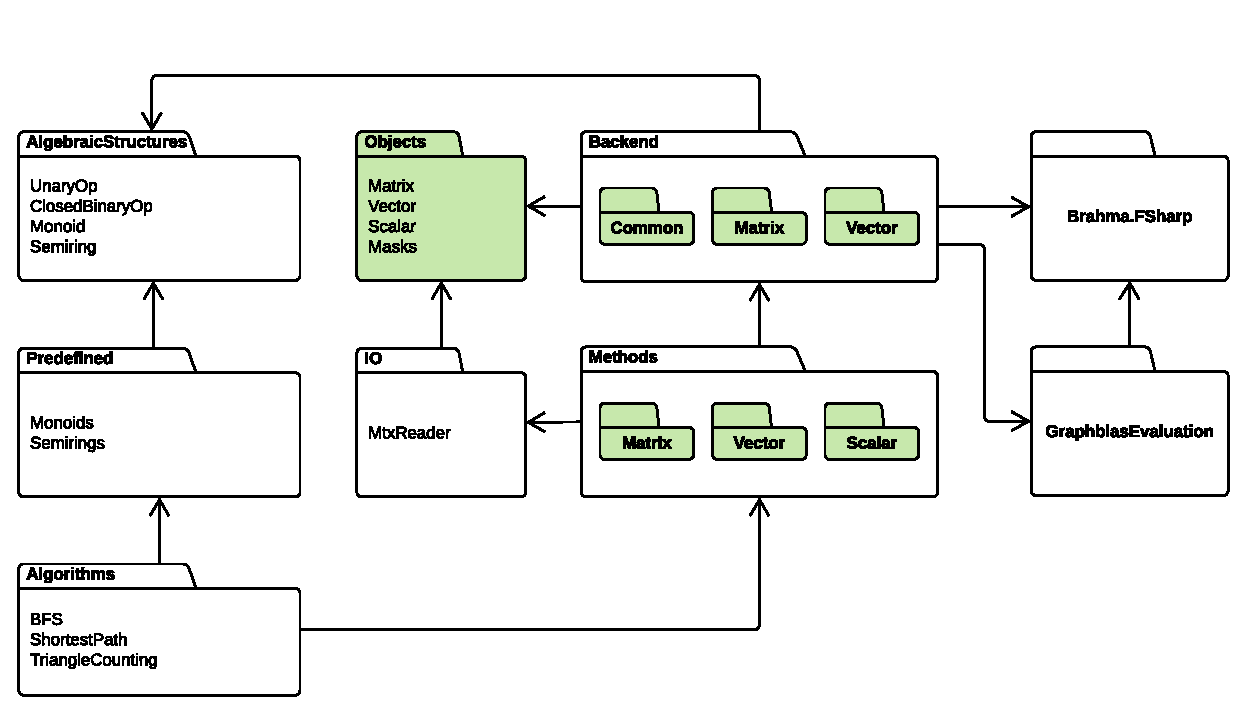
\includegraphics[scale=0.8]{architecture}}
\caption{Общая архитектура предлагаемого решения. Зелёным цветом выделены пакеты, над которыми работал автор.}
\label{architecture}
\end{figure}

\subsection{Примитивы линейной алгебры}
\paragraph{} Из примитивов линейной алгебры реализованы матрица и вектор, представленные в координатном формате, одномерная и двумерная маски, а также скаляр. Представления вышеперечисленных примитивов описаны в пакете Objects.

Координатный формат представления разреженной матрицы\footnote{Статья о разреженной матрице, раздел "Coordinate list (COO)" --- https://en.wikipedia.org/wiki/Sparse\_matrix (дата обращения: 2021-06-07)} подразумевает хранение элементов в виде цепочки троек \((i,j,a)\), где \(i\) --- номер строки, \(j\) --- номер столбца, \(a\) --- значение, находящееся в \(i\)-той строке и в \(j\)-том столбце. Для вектора хранение организовано аналогично. Матрица и вектор, представленные в координатном формате, описаны записями COOMatrix и COOVector соответственно. Запись COOMatrix имеет поля Rows, Columns и Values. В поле Rows хранится массив номеров строк, в Columns --- номеров столбцов, а в Values --- значений. Длины этих массивов всегда равны. Таким образом, отдельную тройку \((i,j,a)\) можно получить, взяв по одному значению из каждого массива, расположенному по фиксированному для каждой тройки индексу.

Полиморфизм относительно конкретной реализации матрицы или вектора реализован посредством размеченных объединений. Конкретная реализация каждой операции линейной алгебры описана в пакетах Backend и Methods. Реализация операций подробно описана в разделе \ref{LinearAlgebraOperations}.

Одномерная маска \(\textnormal{\textbf{m}}=\langle{}N,\{i\}\rangle{}\) определяется размером \(N>0\) и множеством \(\textnormal{\textbf{ind(m)}}\) индексов \(\{i\}\), где \(0\leq{}i<N\). Двумерная маска \(\textnormal{\textbf{M}}=\langle{}M,N,\{(i,j)\}\rangle{}\) определяется количеством строк \(M>0\), столбцов \(N>0\) и множеством \(\textnormal{\textbf{ind(M)}}\) пар \(\{(i,j)\}\), где \(0\leq{}i<M\), \(0\leq{}j<N\). Нетрудно заметить, что одномерные и двумерные маски аналогичны векторам и матрицам соответственно, за исключением того, что маски не имеют значений. Также, на маске определена унарная операция --- взять дополнение. Для одномерной маски \(\textnormal{\textbf{m}}\) дополненная маска \(\textnormal{\textbf{\textlnot{}m}}\) определяется как маска такого же размера, такая что \(\textnormal{\textbf{ind(\textlnot{}m)}}=\{i:0\leq{}i<N,i\notin{}\textnormal{\textbf{ind(m)}}\}\), то есть её множество индексов содержит все возможные элементы, не содержащиеся во множестве индексов изначальной маски. Для двумерной маски дополнение определяется аналогично.

Маска используется для того, чтобы обозначить, какие элементы нужно обрабатывать в операции, а какие --- игнорировать. Применение маски позволяет избежать вычислений значений, которые не требуются в рамках текущей задачи, что обеспечивает оптимизацию вычислений. Также маска позволяет обращаться к конкретным элементам матрицы или вектора, требующимся в данном контексте. Операции линейной алгебры, поддерживающие маску, могут быть выполнены либо с ней, либо без неё. В первом случае вычисления будут производиться над всеми элементами результирующего вектора или матрицы, во втором --- только над отмеченными в данной маске.

Классы Mask1D и Mask2D описывают одномерную и двумерную маски соответственно. В классе Mask1D содержится информация о размере одномерной маски, а также множество индексов, представленное в виде массива. В классе Mask2D хранение организовано аналогично в соответствии с её определением. Если реализовывать операцию "взять дополнение" явно, то применение данной операции к маске, построенной по разреженной матрице, будет возвращать в качестве результата маску, внутри которой будет храниться большое количество избыточной информации. По этой причине вместо этого в классы Mask1D и Mask2D был добавлен флаг isComplemented, отражающий необходимость взять дополнение данной маски перед использованием. Экземпляры классов Mask1D и Mask2D создаются вызовом функций mask или complemented для вектора и матрицы соответственно, реализованных в пакете Methods. Поддержка отсутствия маски реализована с использованием идеи перегрузки функций. Так как перегрузка в явном виде не поддерживается в F\#, были созданы отдельные функции для каждой операции, поддерживающей маску, не принимающие её в качестве аргумента.

Некоторые операции принимают или возвращают единичное значение определённого типа, которым параметризованы эти операции. При этом реализовывать оптимизированные операции, работающие непосредственно с переменной, принадлежащей данному типу, не представляется возможным, так как это потенциально может требовать частого копирования единичного значения из видеопамяти. По этой причине был реализован класс Scalar, позволяющий хранить все единичные значения в видеопамяти и копировать их только по требованию программиста.

\subsection{Операции линейной алгебры}\label{LinearAlgebraOperations}
\paragraph{} В этом разделе будет подразумеваться координатный формат представления матрицы и вектора, если формат не будет уточняться.

Операции могут принимать матрицу, вектор, моноид (запись Monoid из пакета AlgebraicStructures), полукольцо (запись Semiring из того же пакета) и маску. Запись Monoid описывает множество (тип), определённую на нём бинарную ассоциативную операцию и нейтральный относительно этой операции элемент, принадлежащий этому множеству, то есть имеющий данный тип. Запись Semiring описывает пару: коммутативный моноид и мультипликативная операция. Таким образом, записи Monoid и Semiring определяют контекст, в котором требуется выполнить операцию.

\subsubsection{Поэлементное сложение матриц и векторов}
\paragraph{}В рамках поэлементного сложения матрица и вектор, представленные в координатном формате хранения, могут быть рассмотрены как ничем не отличающиеся друг от друга примитивы линейной алгебры. Как уже было упомянуто ранее, матрица представляется в виде трёх массивов: номеров строк, номеров столбцов и значений. Пару, состоящую из первых двух массивов, можно воспринимать как один массив индексов. При этом форма представления ничем не будет отличаться от представления вектора. Поэтому рассмотрим далее только поэлементное сложение векторов.

Работа алгоритма состоит из следующих этапов.
\begin{enumerate}
    \item Слить массивы индексов векторов в один с сохранением упорядоченности элементов.
    \item Отметить повторяющиеся индексы в получившемся массиве.
    \item Посчитать итоговую позицию каждого неповторяющегося индекса в получившемся массиве.
    \item Перенести неповторяющиеся данные в результирующий массив индексов.
\end{enumerate}

Таким образом, в результате получится упорядоченный массив, представляющий собой объединение двух исходных массивов как объединение множеств. Разделение алгоритма на вышеперечисленные этапы позволяет достичь параллелизма при его исполнении.

Помимо массива индексов требуется получить результирующий массив значений. Если значение встречается в паттерне только одного из векторов, оно будет складываться с нулём. Для избежания лишних вычислений, по аддитивному свойству нуля (\(\forall{}a\;\;a+0=0+a=a\)) это значение сразу может быть записано в результирующий массив. Таким образом, складывать друг с другом требуется только пары значений под одинаковыми индексами. Над массивами значений производятся те же операции, что и над массивами векторов, за исключением того, что во время второго этапа дополнительно производится сложение пар элементов под одинаковыми индексами. При этом результат сложения записывается вместо того значения в паре, которое будет записано в результирующий массив.

Первый этап сложения представляет собой алгоритм Merge Path \cite{OdedGreen}. Этот алгоритм можно рассматривать как модификацию типичного однопоточного слияния двух упорядоченных массивов в один упорядоченный. При этом он обладает массовым параллелизмом. Идея этого алгоритма проиллюстрирована на рисунке \ref{merge_path}. На осях расположены два массива \(A\) и \(B\), которые требуется слить. На пересечениях \(i\)-той строки с \(j\)-тым столбцом находится 1, если \(A[i] < B[j]\), или 0 иначе. Упорядоченность обоих массивов порождает, неформально говоря, лестницу, отделяющую клетки со значением 1 от клеток со значением 0. Заметим, что количество диагоналей в таблице равно сумме размеров массивов \(A\) и \(B\). Пронумеруем диагонали таблицы. По тому, где и как \(i\)-тая диагональ пересекается с полученной лестницей, можно однозначно определить, каким будет \(i\)-тое значение результирующего массива. Заметим также, что для каждой конкретной диагонали не требуется никакой информации о других диагоналях. Таким образом, для каждой диагонали параллельно можно найти бинарным поиском место пересечения с лестницей и, следовательно, значение в результирующем массиве.

\begin{figure}[h]
\center{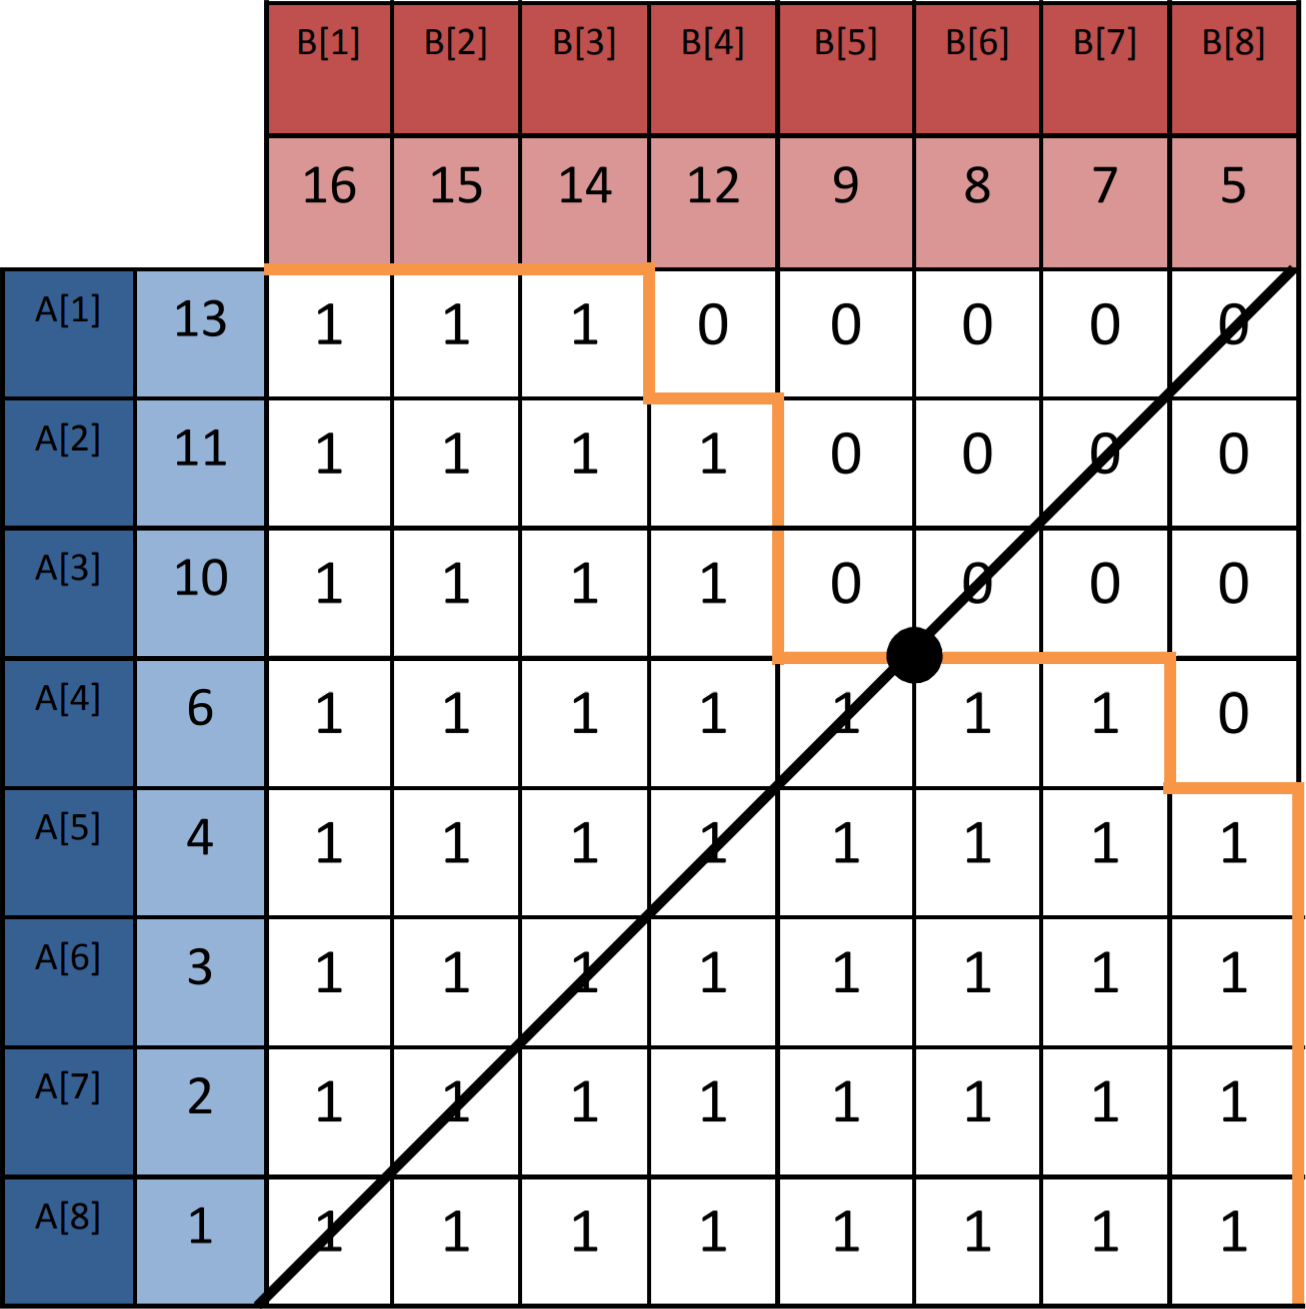
\includegraphics[scale=0.3]{merge_path}}
\caption{Демонстрация концепции алгоритма Merge Path. Изображение взято из статьи \cite{OdedGreen}}
\label{merge_path}
\end{figure}

Второй этап заключается в проверке повторяющихся элементов получившегося массива \(C\). Создаётся вспомогательный массив, в котором на \(i\)-той позиции записывается 1, если \(C[i] \neq C[i-1]\), и 0 иначе.

В третьем этапе к вспомогательному массиву применяется алгоритм вычисления префиксных сумм\footnote{Статья с описанием алгоритма вычисления префиксных сумм --- https://developer.nvidia.com/gpugems/gpugems3/part-vi-gpu-computing/chapter-39-parallel-prefix-sum-scan-cuda (дата обращения: 2021-06-08)}. Для вспомогательного массива \(\langle a_0, a_1, a_2, a_3, \dots\rangle\) результатом третьего этапа будет массив \(\langle 0, a_0, a_0 + a_1, a_0 + a_1 + a_2, \dots\rangle\).

После третьего этапа из вспомогательного массива получается массив \(E\), такой что \(i\)-тый элемент результирующего массива будет равен \(D[E[i]]\), где \(D\) --- массив, полученный на первом этапе. В соответствии с этой формулой на четвёртом этапе заполняются результирующие массивы.

\subsubsection{Сокращение вектора при помощи аддитивной операции}
\paragraph{}Операция сокращения вектора возвращает скаляр, хранящий в себе сумму всех элементов вектора. Таким образом, для её реализации достаточно взять массив значений вектора и вычислить сумму всех его элементов.

Вычисление суммы всех элементов массива было реализовано с помощью упрощения алгоритма вычисления префиксных сумм массива путём отбрасывания лишних инструкций. Изначально массив делится на множество участков, в каждом из которых эффективно вычисляется локальная сумма этого участка и записывается в дополнительный массив. Таким образом, после этого этапа остаётся решить ту же задачу, но уже для вспомогательного массива, длина которого в \(n\) раз меньше, чем у изначального, где \(n\) --- количество элементов в одном участке. Этот же шаг применяется итеративно к каждому новому массиву, пока длина очередного массива не станет равной 1. На основе указателя на первое значение в этом массиве создаётся запись Scalar и возвращается в качестве выходной переменной. В целях экономии памяти, после того, как количество дополнительных массивов становится равным двум, новые массивы не создаются. Вместо этого значениями заполняется старый, после чего указатели на два дополнительных массива меняются местами.

\subsubsection{Запись вектора и скаляра в вектор через маску}
\paragraph{}Алгоритм записи вектора (вектор-аргумент) через маску в другой вектор (вектор-цель) состоит из следующих этапов.
\begin{enumerate}
    \item Фильтрация вектора-аргумента через маску.
    \item Слияние полученного вектора с вектором-целью.
\end{enumerate}

Для того чтобы получить вектор, профильтрованный через маску, нужно отбросить у него те элементы, индексы которых не содержатся в маске. Это реализовано аналогично алгоритму поэлементного сложения с той лишь разницей, что в последнем используется объединение индексов как множеств, в отличие от данного алгоритма, в котором используется их пересечение как множеств. Пересечение получится, если взять те элементы, которые отбрасывались в алгоритме поэлементного сложения. При этом элементы, содержащиеся в маске, но не содержащиеся в векторе, также добавляются в профильтрованный вектор со специальной меткой, так как эти элементы должны быть удалены из вектора-цели.

Второй этап записи вектора также аналогичен алгоритму поэлеметного сложения. Отличие состоит в том, что вместо операции сложения производится операция записи значения из отфильтрованного вектора-аргумента. Помимо этого значение со специальной меткой удаляется из результирующего вектора, то есть помечается нулем во вспомогательном массиве, для которого вычисляются префиксные суммы.

Запись скаляра в вектор через маску является частным случаем записи вектора. Таким образом, реализация этой операции аналогична вышеописанной.

\section{Результаты}
\paragraph{}В данном разделе описаны результаты сравнения с существующим аналогом и сделанные на их основе выводы.

\subsection{Сравнение с аналогом}
\paragraph{}В качестве аналога для сравнения была выбрана библиотека\\ SuiteSparse. Сравнение производилось на примере поэлементного сложения двух матриц. В качестве контекста было выбрано полукольцо с типом, представляющим собой 32-битные числа с плавающей запятой, и стандартным сложением для этого типа. Матрицы, на которых тестировались алгоритмы, были выбраны из множества, предоставляемого SuiteSparse Matrix Collection \cite{DavidTimothy}. Каждая матрица, будучи квадратной, складывалась с собой, возведённой заранее в квадрат. Характеристики выбранных матриц отражены в таблице \ref{matrices}. Характеристики ПК, на котором производилось сравнение: Ubuntu 20.04, Intel core i7-4790 CPU, 3.6GHz, DDR4 32Gb RAM и GeForce GTX 1070 GPU, 8Gb VRAM. Сравнение проводилось с помощью библиотеки BenchmarkDotNet\footnote{Репозиторий библиотеки BenchmarkDotNet --- https://github.com/dotnet/BenchmarkDotNet (дата обращения: 2021-11-13)}. Для каждой матрицы алгоритм запускался по 5 итераций. Учитывалось время копирования всех данных в видеопамять.
 
\begin{table}[h]
\center{}

\begin{tabular}{ | c | c | c | c | }
\hline
Название & Размер & \parbox[c][2.5cm][t]{3cm}{\center{Количество ненулевых элементов}} & \parbox[c][3.5cm][t]{3cm}{\center{Количество ненулевых элементов у возведённой в квадрат}} \\ \hline
luxembourg\_osm & 114599 & 119666 & 4582 \\ \hline
belgium\_osm & 1441295 & 1549970 & 148316 \\ \hline
wiki-Talk & 2394385 & 5021410 & 42937 \\ \hline
cit-Patents & 3774768 & 16518948 & 1222 \\ \hline
\end{tabular}

\caption{Матрицы, на которых производилось сравнение}
\label{matrices}
\end{table}

Результаты сравнения приведены в таблицах \ref{graphblas-sharp} и \ref{suitesparse}.

\begin{table}[h]
\center{}

\begin{tabular}{ | c | c | c | c | }
\hline
Название & Среднее, мс & Стандартное отклонение, мс \\ \hline
luxembourg\_osm & 37.2 & 0.25 \\ \hline
belgium\_osm & 80.98 & 0.24 \\ \hline
wiki-Talk & 125.85 & 1.92 \\ \hline
cit-Patents & 504.51 & 3.4 \\ \hline
\end{tabular}

\caption{Результаты замеров для библиотеки GraphBLAS-sharp}
\label{graphblas-sharp}
\end{table}

\begin{table}[h]
\center{}

\begin{tabular}{ | c | c | c | c | }
\hline
Название & Среднее, мс & Стандартное отклонение, мс \\ \hline
luxembourg\_osm & 9.81 & 5.49 \\ \hline
belgium\_osm & 46.59 & 4.52 \\ \hline
wiki-Talk & 53.51 & 4.22 \\ \hline
cit-Patents & 263.47 & 48.02 \\ \hline
\end{tabular}

\caption{Результаты замеров для библиотеки SuiteSparse}
\label{suitesparse}
\end{table}

Из результатов видно, что предлагаемое решение на данном этапе на больших матрицах проигрывает аналогичному примерно в 2 раза.

Было выяснено, что библиотека Brahma.FSharp не позволяет выделять память сразу в видеопамяти, а требует выделять память на основном CPU, используемом для настройки выполнения, и затем копировать ее в видеопамять. В связи с этим образовываются накладные расходы на копирование вспомогательных данных в видеопамять. Время, затрачиваемое на копирование данных, представлено в таблице \ref{time}.

\begin{table}[h]
    \center{}
    
    \begin{tabular}{ | c | c | c | }
    \hline
    Название матрицы & Среднее время копирования данных, мс \\ \hline
    luxembourg\_osm & 6.57 \\ \hline
    belgium\_osm & 36.04 \\ \hline
    wiki-Talk & 85.52 \\ \hline
    cit-Patents & 353.38 \\ \hline
    \end{tabular}
    
    \caption{Результаты замеров времени копирования вспомогательных данных}
    \label{time}
    \end{table}

\subsection{Выводы}
\paragraph{}В результате сравнения с аналогичным решением были сформулированы следующие выводы.

\begin{itemize}
    \item Снижение накладных расходов осуществимо путём модифицирования библиотеки Brahma.FSharp.
    \item С учётом переносимости и высокоуровневого интерфейса предлагаемое решение жизнеспособно.
\end{itemize}
% \paragraph{}Выяснение причин низкой производительности решения является затруднительной задачей, так как высокоуровневый язык с управляемой памятью с использованием OpenCL усложняет профилирование кода. Тем не менее, были сформулированы предположительные причины, перечисленные ниже.

% \begin{itemize}
%     \item Длительное компилирование кода ядер во время исполнения.
%     \item Большие накладные расходы при копировании данных между управляемой, неуправляемой и видеопамятью.
%     \item Использование недостаточно оптимальных алгоритмов ввиду ограничения на произвольные типы (а именно, отсутствие поддержки атомарных операций для них).
% \end{itemize}

\section*{Заключение}
\paragraph{} В ходе выполнения данной работы были достигнуты следующие результаты.
\begin{itemize}
    \item Реализована на языке F\# архитектура таких описанных в стандарте GraphBLAS примитивов линейной алгебры, как одномерная и двумерная маски, матрица и вектор, представленные в координатном формате, а также скаляр.
    \item Реализованы на языке F\# такие операции линейной алгебры над матрицами и векторами, представленными в координатном формате, с поддержкой OpenCL, как поэлементное сложение матриц/векторов, сокращение вектора при помощи аддитивной операции, запись вектора/скаляра в другой вектор через маску.
    \item Произведено сравнение с существующим аналогом по производительности и выявлены пути к оптимизации существующего решения.
\end{itemize}

Код доступен в репозитории\footnote{Ответвление от исходного репозитория библиотеки с окончательной версией реализации стандарта GraphBLAS --- https://github.com/artemgl/GraphBLAS-sharp (дата обращения: 2021-06-08).}, размещённом на веб-сервисе GitHub.

\bibliographystyle{ugost2008ls}
\bibliography{diploma.bib}

\end{document}